\documentclass[twoside]{scrartcl}
\usepackage[utf8]{inputenc}
\usepackage[T1]{fontenc}
\usepackage{lmodern}
\usepackage{latexsym}
\usepackage{amsfonts}
\usepackage{amssymb}
\usepackage{fancyhdr,lastpage}
\usepackage{listings}
\usepackage{hyperref}
\usepackage{amsmath}
\usepackage{graphicx}
\usepackage{geometry}
\usepackage[ngerman]{babel}
\geometry{hmargin={1cm,1cm},vmargin={2.4cm,3cm}}
\usepackage{comment}
\newcommand{\llfloor}{\left\lfloor}
\newcommand{\rrfloor}{\right\rfloor}
\setlength{\headheight}{20pt}
\pagestyle{fancy}
\fancyhf{}
\fancyhead[L]{Interim Report 1}
\fancyhead[C]{Fabian Hirschmann, Michael Markert}
\fancyhead[R]{\today}
\fancyfoot[C]{Page \thepage\ of \pageref{LastPage}}
\begin{document}
\noindent An overview of the currently implemented algorithms can be found
in this report.
\section{Cleaning Algorithms}
\subsection{Deduplication Algorithm}
Merge nodes with same location using mongodb's MapReduce.

\section{Merging Algorithms}
\subsection{Angle-based Merging Algorithm}
Algorithm for merging parallel train tracks.
\begin{lstlisting}[mathescape]
for each intersection:
    if the angle between two neighbors $n_1$ and $n_2$ is $< \varepsilon$:
        (if the length of the line segment $n_1$ $n_2$ is $<  \delta$:)
            replace $n_1$ and $n_2$ with a node located at the midpoint of the line segment
\end{lstlisting}

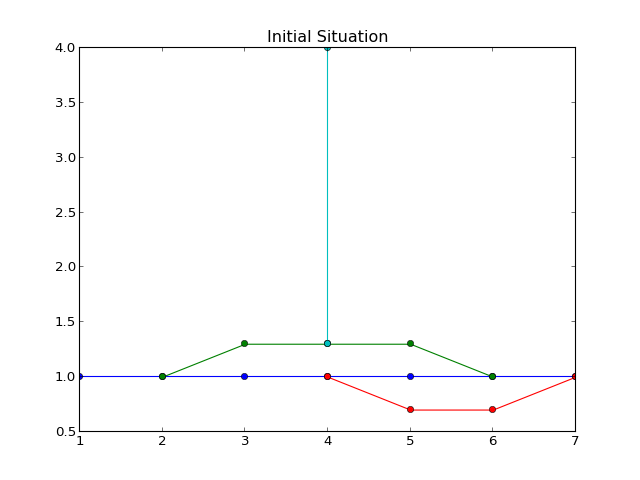
\includegraphics[scale=0.48]{comb-1.png}
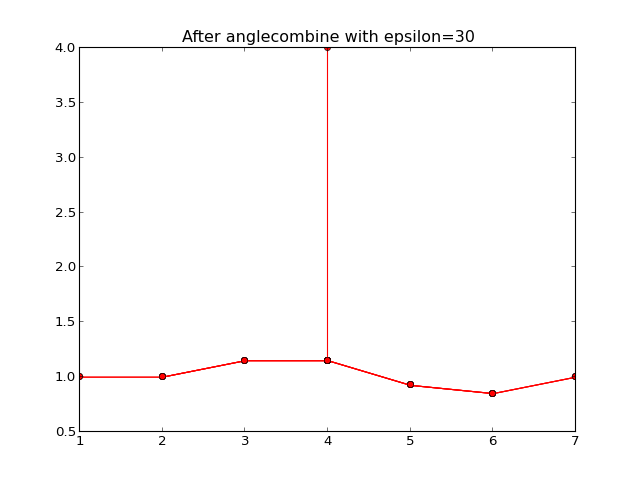
\includegraphics[scale=0.48]{comb-2.png}

\section{Network Segmentation}
\subsection{Intersection/Endpoint Segmentation Algorithm}
Segments a network graph. Segments are defined by its bounds, which are
either endpoints or intersections.
\newpage

\section{Line Simplification}
\subsection{Angle-based reduction}
Removes a point if the angle between a point and its two neighbors
is greater than a threshold value.\\
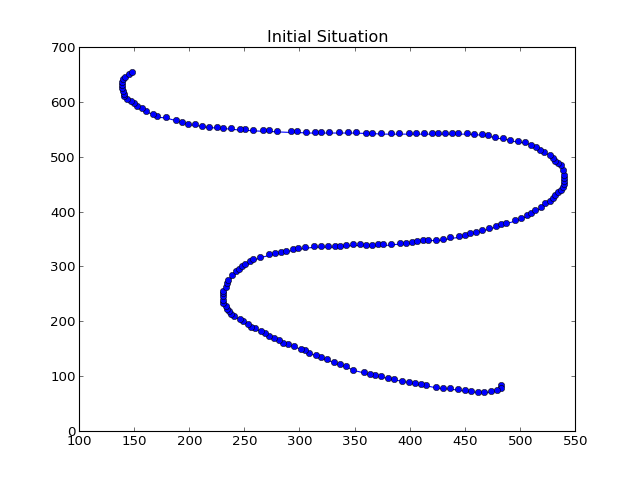
\includegraphics[scale=0.48]{simp-1.png}
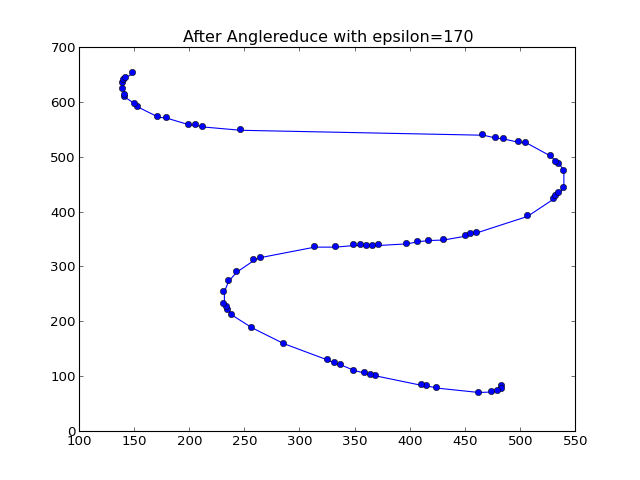
\includegraphics[scale=0.48]{simp-2.png}
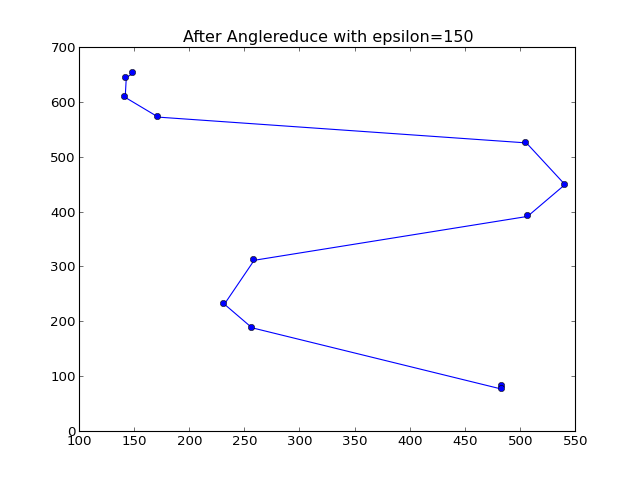
\includegraphics[scale=0.48]{simp-3.png}\\
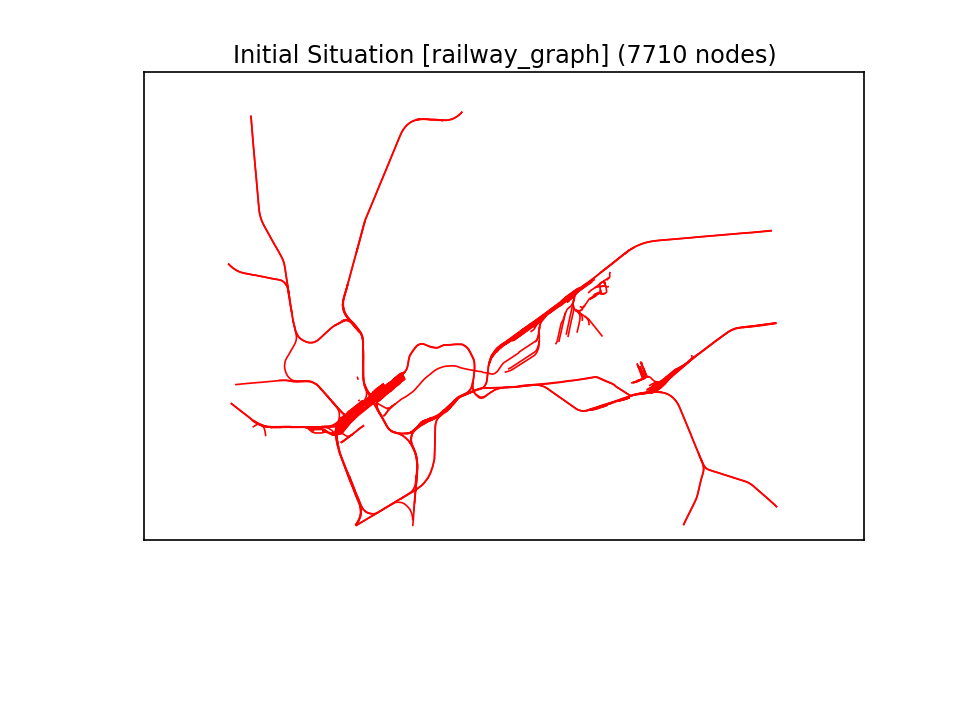
\includegraphics[scale=0.49]{anglered-1.png}
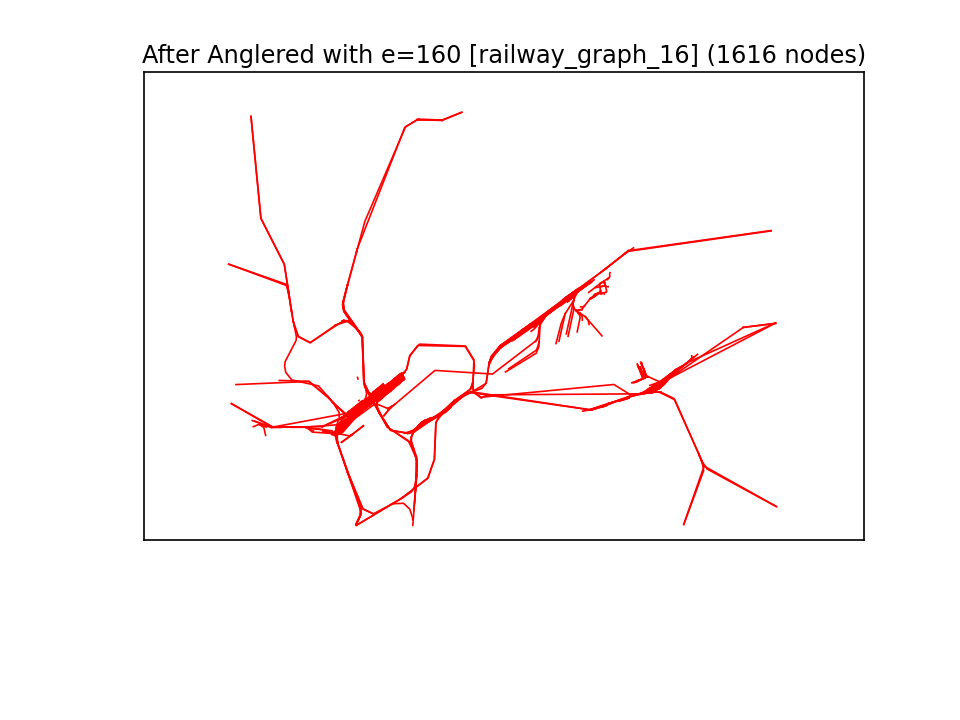
\includegraphics[scale=0.49]{anglered-2.png}

\subsection{Ramer-Douglas-Peucker Algorithm}
Based on maximum threshold distance between a point and the approximated
line segment.\\
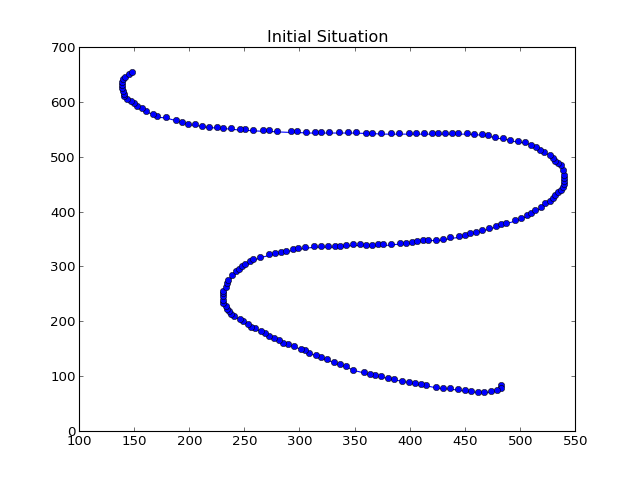
\includegraphics[scale=0.48]{simp-4.png}
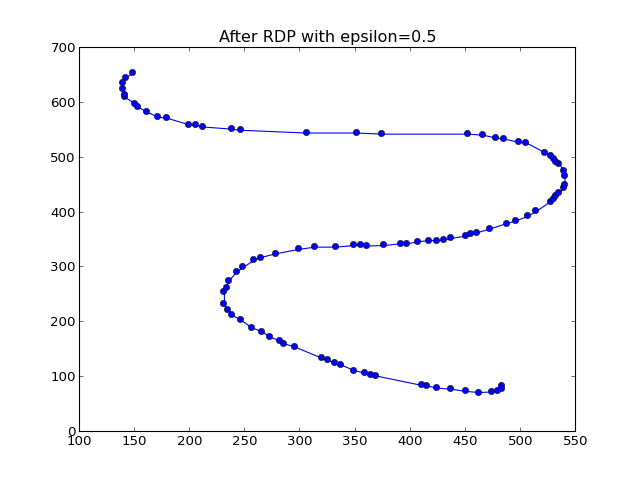
\includegraphics[scale=0.48]{simp-5.png}
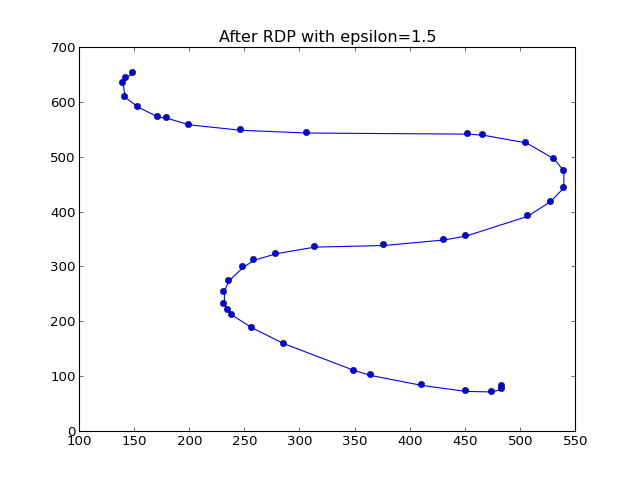
\includegraphics[scale=0.48]{simp-6.png}\\
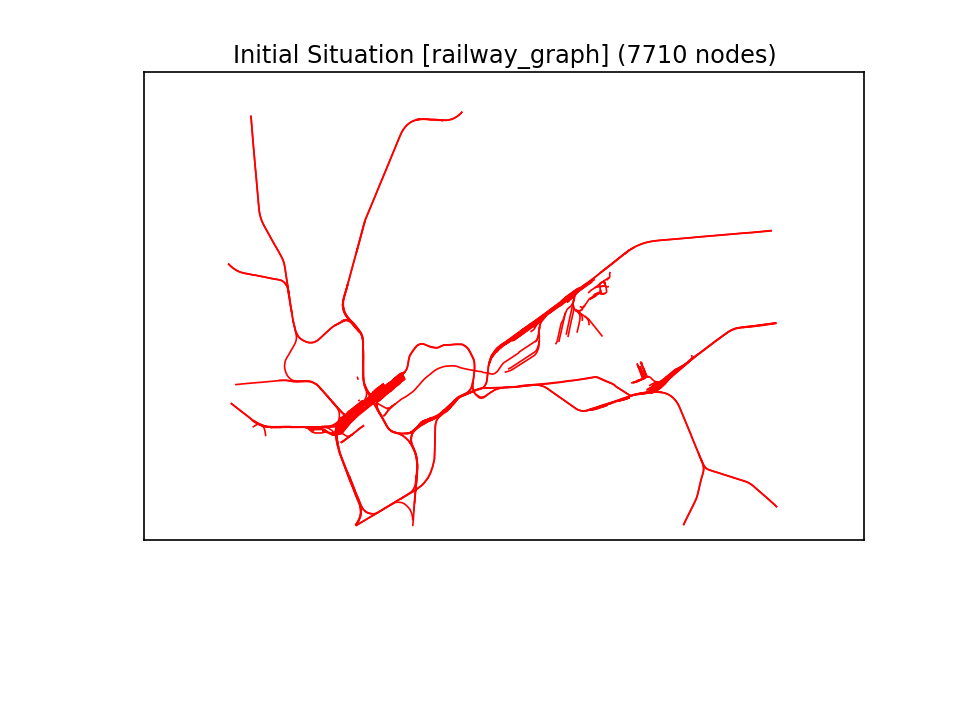
\includegraphics[scale=0.49]{rdprg-1.png}
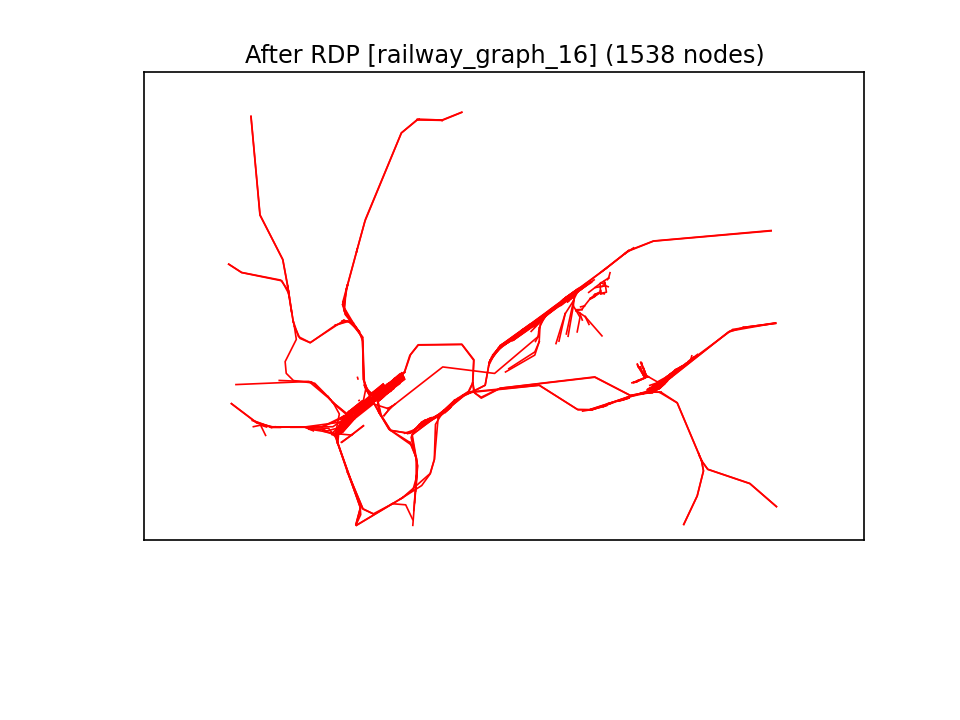
\includegraphics[scale=0.49]{rdprg-2.png}

\section{Other achievements}
\begin{itemize}
    \item Sphinx documentation
\end{itemize}

\section{Todo}
\begin{itemize}
    \item Mercator projection before applying simplification algorithms
\end{itemize}

\section{Open Questions}
\begin{itemize}
    \item Node distance: Great-circle distance? Euclidean distance on mercator projection?
    \item Command Line Interface user-friendly?
    \item Selection of points representing stations?
    \item layout of \texttt{Stations.txt} and \texttt{sgrv.csv}
\end{itemize}

\newpage
\section{Appendix}
Ramer-Douglas-Peucker visualization:\\
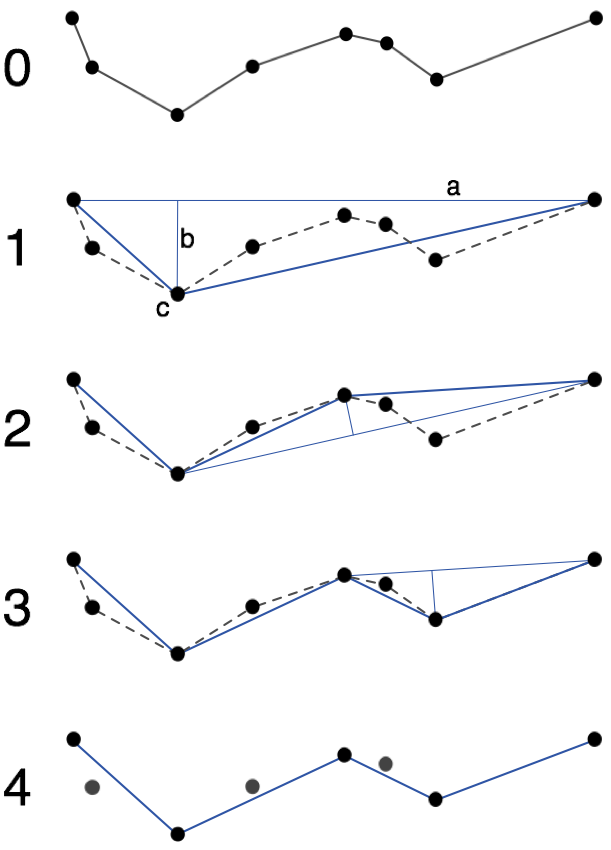
\includegraphics[scale=0.6]{rdp.png}
\end{document}
